\section{LocARNA}

\begin{frame}[c]{LocARNA - basic information}
    \begin{itemize}[<+(1)->]
        \item Extensive Caching (Dynamic Programming) + Pruning
        \item {\bf Runtime} $O(n^4)$
        \item {\bf Space} $O(n^4)$
        \item Web Interface
        \item Developed at the University of Freiburg
    \end{itemize}
\end{frame}

%     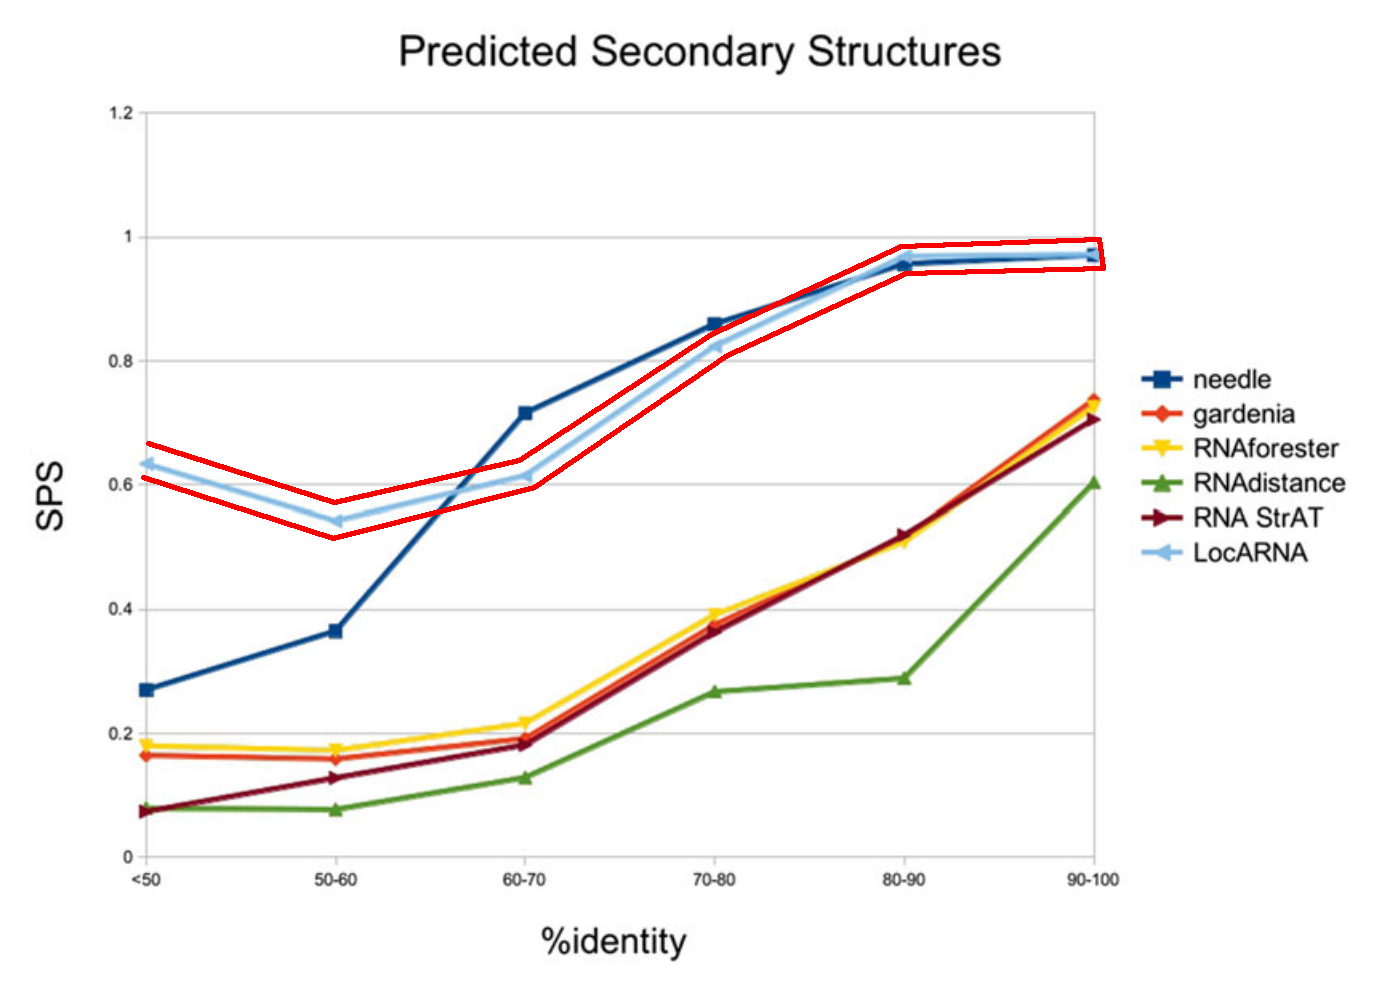
\includegraphics[width=\textwidth]{predicted_LocARNA}


\begin{frame}[c]{LocARNA - Procedure}
    \begin{itemize}[<+(1)->]
    \item Where can arcs happen? And how likely are they?
    \item Building own likely secondary structures
    \item Aligning between secondary structures
    \item Using {\bf one} relative path Matrix
    \item Last: 'looking up' optimal alignment
    \end{itemize}
\end{frame}


\begin{frame}[c]{LocARNA - Where can arcs happen? \\ And how likely are they?}
    \begin{overprint}
    \onslide<1>\centering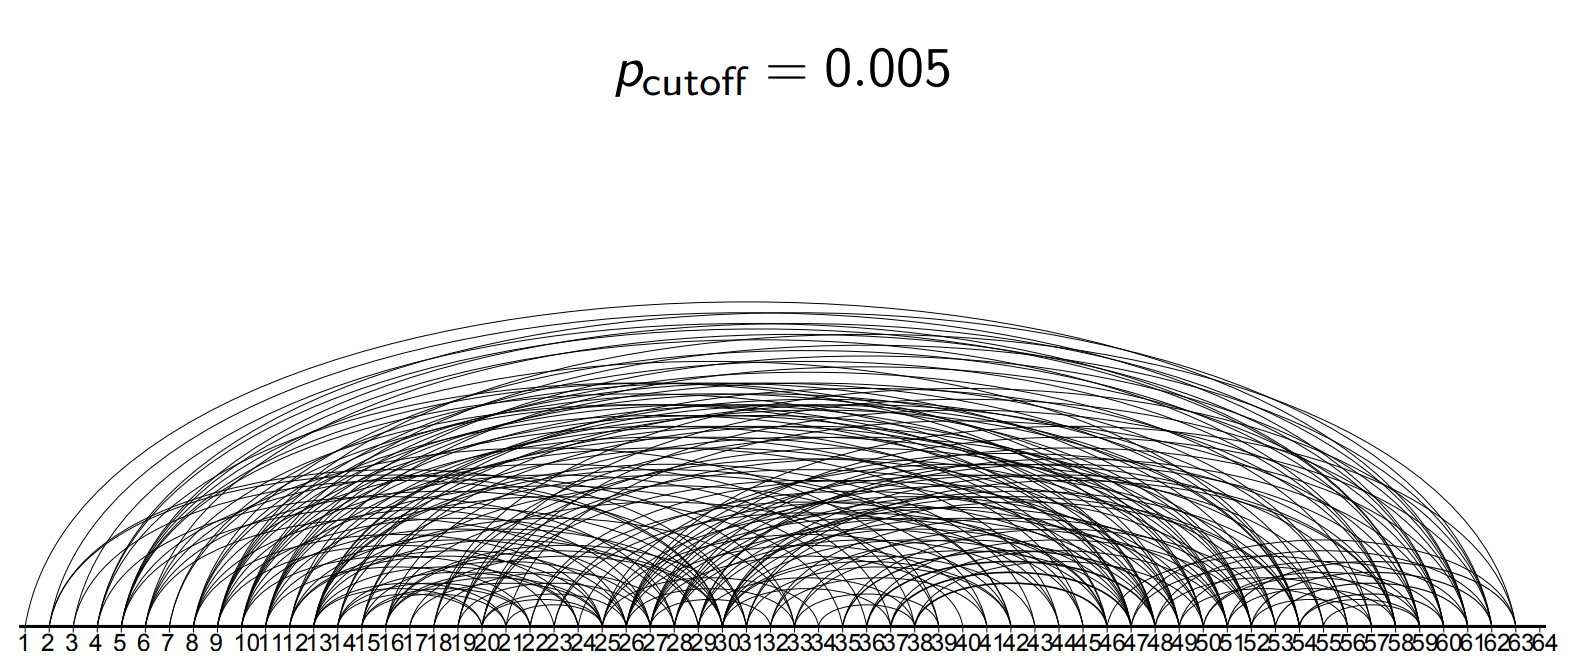
\includegraphics[width=\textwidth]{cutoff_0005}
    \onslide<2>\centering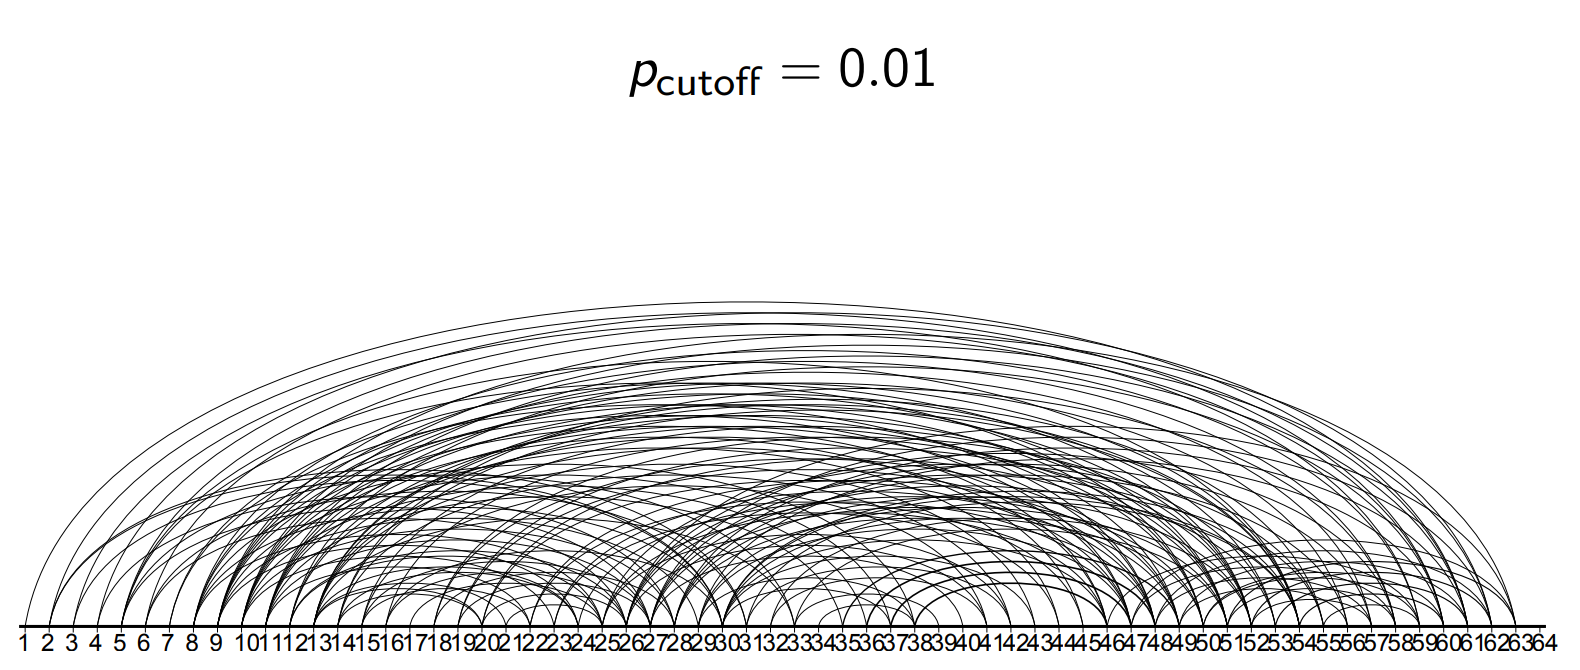
\includegraphics[width=\textwidth]{cutoff_001}
    \onslide<3>\centering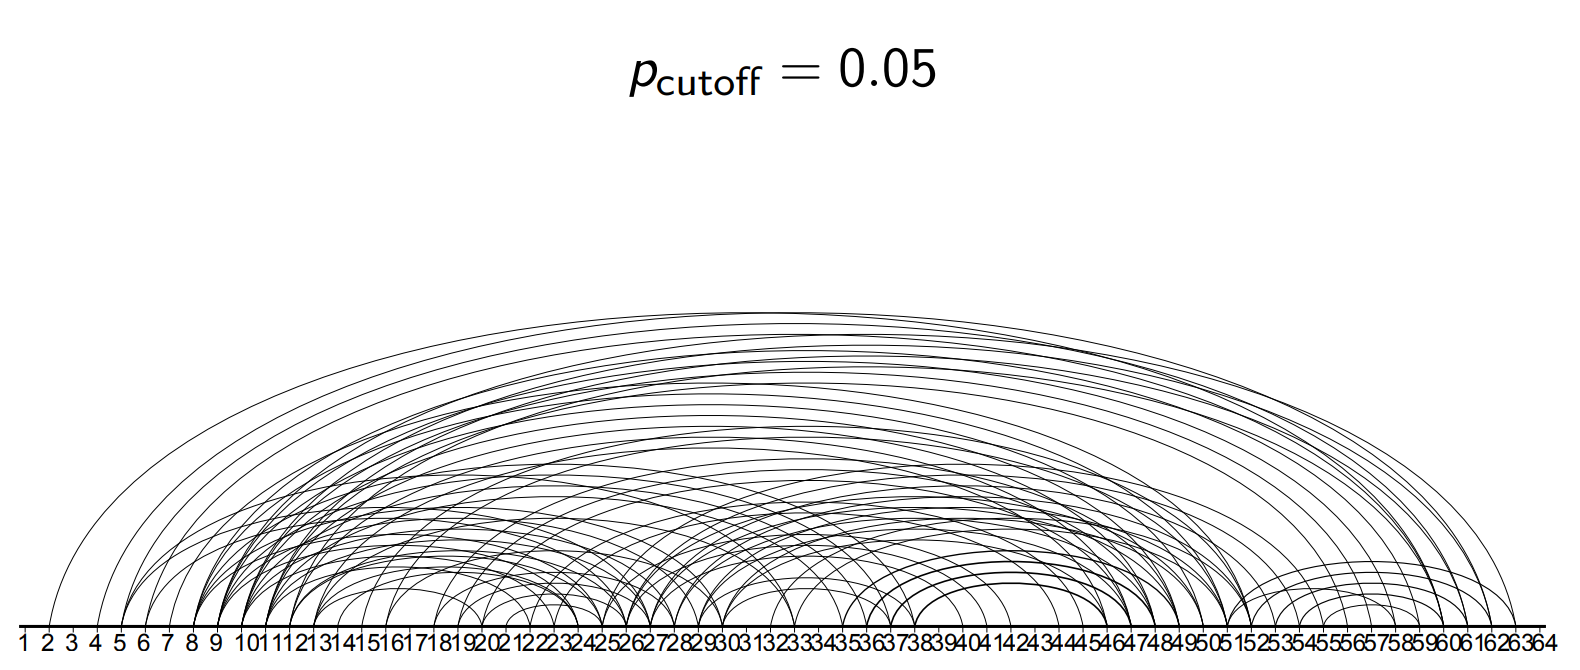
\includegraphics[width=\textwidth]{cutoff_005}
    \onslide<4>\centering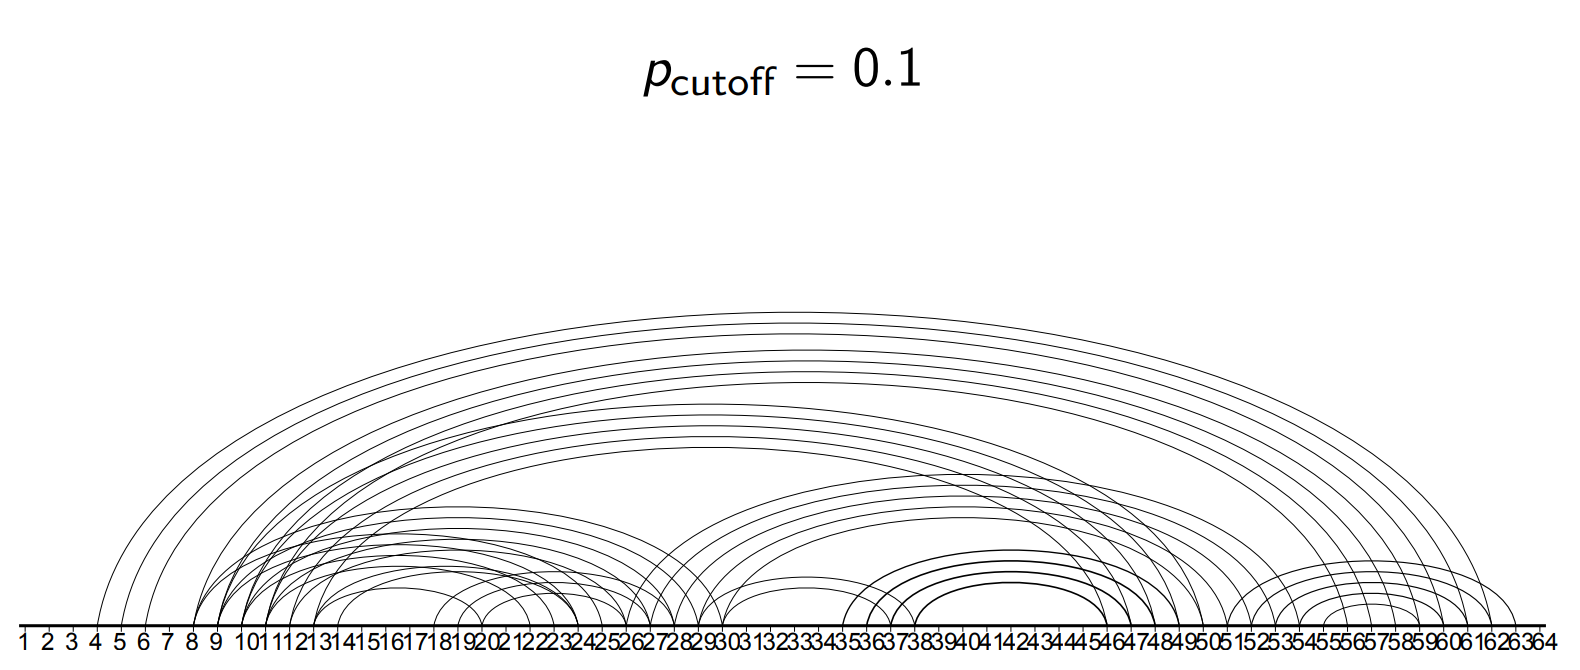
\includegraphics[width=\textwidth]{cutoff_01}
    \end{overprint}
\end{frame}


\begin{frame}[c]{LocARNA - Matrices}
    \begin{overprint}
    \onslide<1>\centering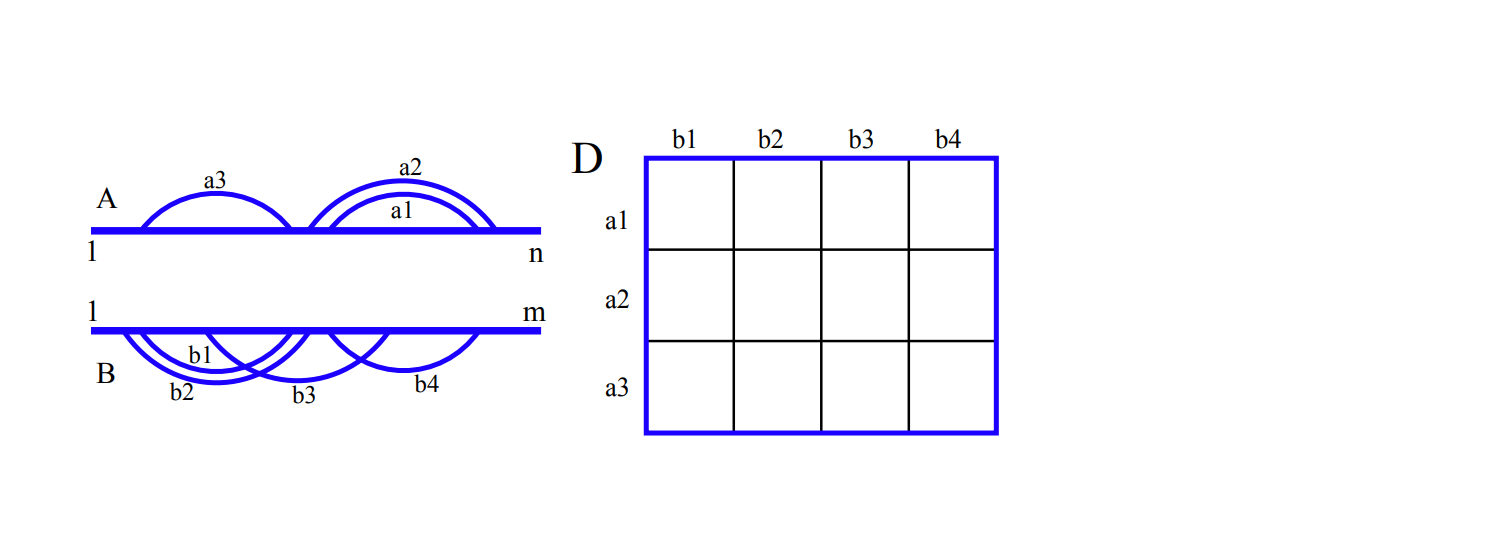
\includegraphics[width=\textwidth]{locarnamatrices0}
    \onslide<2>\centering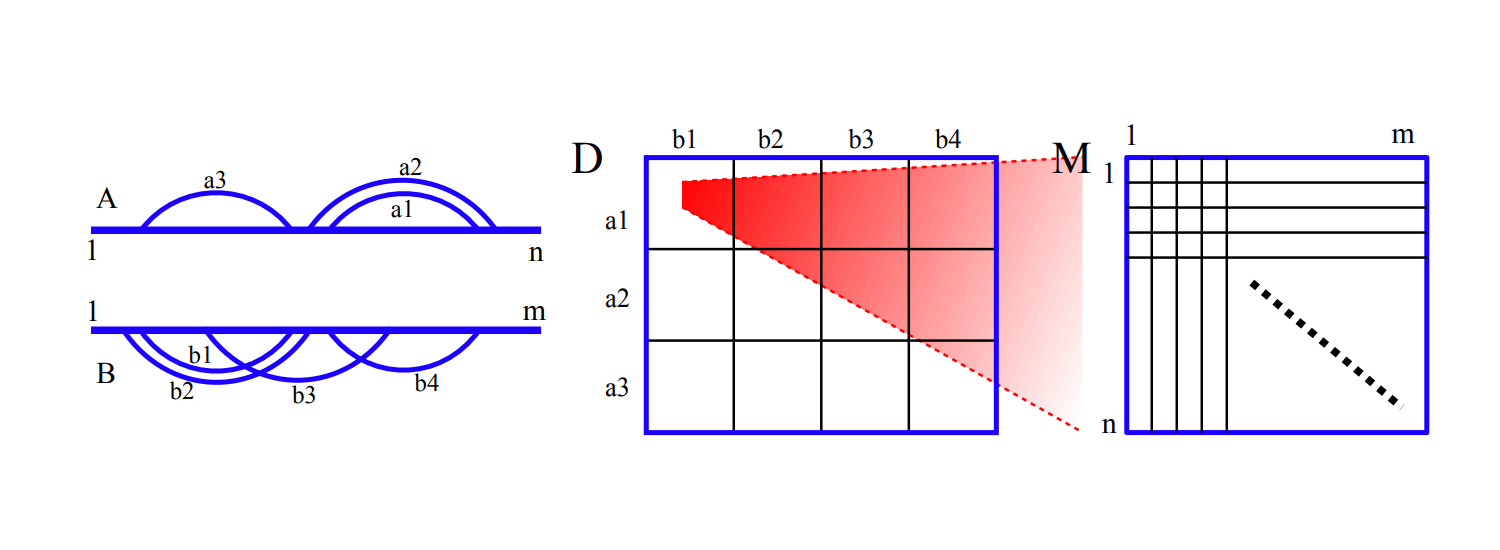
\includegraphics[width=\textwidth]{locarnamatrices1}
    \onslide<3>\centering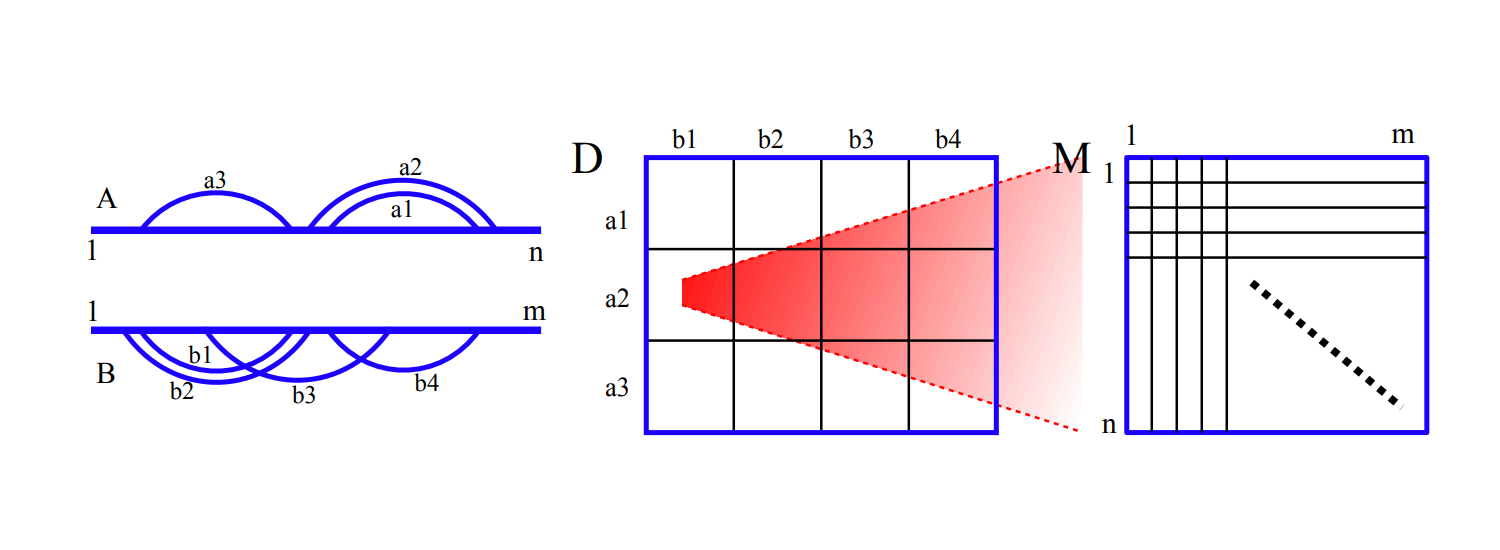
\includegraphics[width=\textwidth]{locarnamatrices2}
    \end{overprint}
\end{frame}

\begin{frame}[c]{LocARNA - Aligning between secondary structures}
    \Large
    Cases:
    \begin{itemize}[<+(1)->]
    \item Base match
    \item Base insertion
    \item Base deletion
    \item Base \textbf{pair} match
    \end{itemize}
\end{frame}



\begin{frame}[c]{LocARNA - Aligning between secondary structures}
    \center
    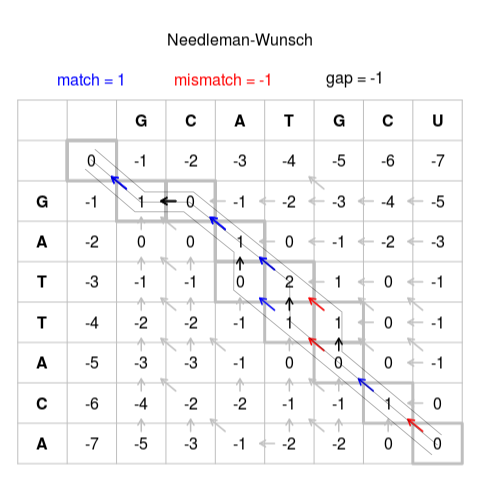
\includegraphics[width=0.73\textwidth]{Needleman-Wunsch_pairwise_sequence_alignment}
\end{frame}


\begin{frame}[c]{LocARNA - Demonstration}
    \center
    
\includegraphics[width=0.5\textwidth]{Arcs_example}
\end{frame}


\begin{frame}[standout]
    Demo Time!
\end{frame}

\begin{frame}[c]{LocARNA - Final actual Alignment}
    \center
    \begin{overprint}
        \only<2>{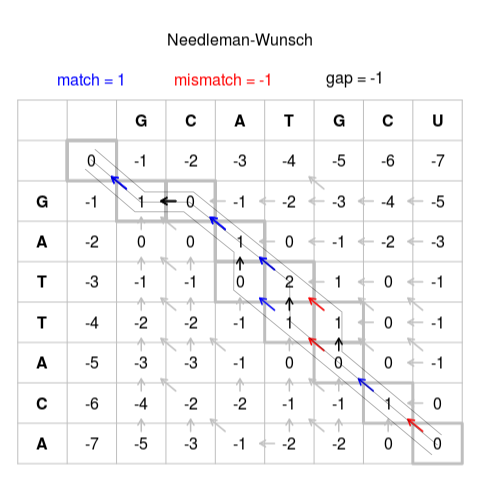
\includegraphics[width=0.73\textwidth]{Needleman-Wunsch_pairwise_sequence_alignment}}
        \only<1>{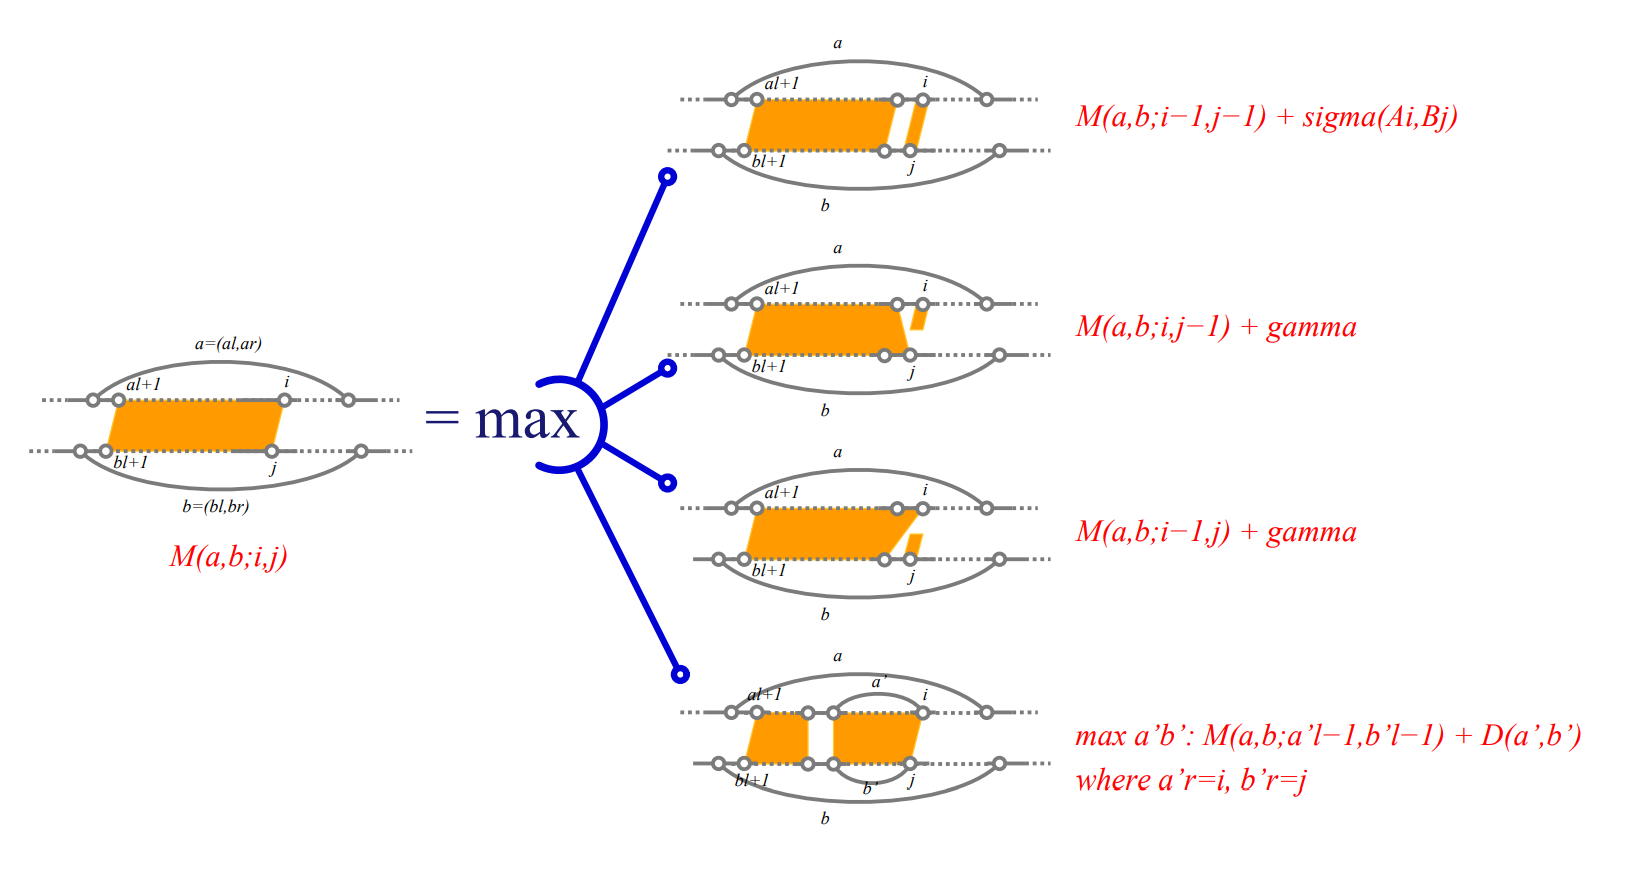
\includegraphics[width=\textwidth]{locarna_formula}}
    \end{overprint}
\end{frame}


% lingering questions:
% - if there's arcs a10 and a14 being locally different but the same, will
%   there be two different places for them in D? in M?
% -



